\section{Resultados e discussão}\label{sec-resultados}

Como dito anteriormente, foram feitos dois experimentos de classificação
de papéis semânticos. O primeiro envolve uma classificação binária (Arg0
e Arg1); já o segundo aborda uma classificação multiclasse com cinco
rótulos (Arg0, Arg1, Arg2, Arg3 e Arg4). Na \Cref{tab-03}, apresentamos os
resultados obtidos, considerando as medidas P, R, MF e A.

\begin{table}[htbp]
  \centering 
  \begin{threeparttable}
  \caption{Resultados para os dois experimentos de classificação.}
  \label{tab-03}
  \begin{tabular}{*{9}{l}}
  \toprule
  \multirow{2}{*}{CLASSES} & \multicolumn{8}{c}{EXPERIMENTOS} \\
    & \multicolumn{4}{c}{1º experimento (Arg0 e Arg1)} & \multicolumn{4}{c}{2º experimento (Arg0 a Arg4)} \\
    & P & R & MF & A & P & R & MF & A \\
  Arg0 & 0,83 & 0,82 & 0,82 & 0,85 & 0,82 & 0,79 & 0,81 & 0,76 \\
  Arg1 & 0,88 & 0,89 & 0,88 & 0,85 & 0,77 & 0,84 & 0,80 & 0,76 \\
  Arg2 &  -   &   -  &   -  &  -   & 0,40 & 0,32 & 0,36 & 0,76 \\
  Arg3 &  -   &   -  &   -  &  -   & 0,33 & 0,14 & 0,20 & 0,76 \\
  Arg4 &  -   &   -  &   -  &  -   & 1,00 & 0,20 & 0,33 & 0,76 \\
  \bottomrule
  \end{tabular}
  \source{Elaborado pelos autores.}
  \end{threeparttable}
\end{table}

Para o primeiro experimento, os resultados mostram um desempenho
equilibrado entre as duas classes. As métricas P, R e MF para Arg0 são,
respectivamente, 83\%, 82\% e 82\%, enquanto para Arg1 são 88\%, 89\% e
88\%. Esses resultados indicam um classificador bem balanceado,
sugerindo que o modelo consegue distinguir bem entre essas duas classes.

Por haver um aumento de classes, já era esperado um desbalanceamento na
performance do modelo entre as diferentes classes, no segundo
experimento. Para as classes Arg0 e Arg1, os resultados são semelhantes
aos do primeiro experimento, com MF de 81\% e 80\%, respectivamente. No
entanto, para as outras classes (Arg2, Arg3 e Arg4), as métricas são
significativamente mais baixas.

Para a classe Arg2, as medidas P, R e MF são 40\%, 32\% e 36\%,
respectivamente. A classe Arg4 apresenta uma precisão perfeita (100\%),
mas uma revocação extremamente baixa (20\%), resultando em uma MF de
apenas 33\%. A classe Arg3 também apresenta baixos valores em todas as
métricas, com precisão, revocação e medida F de 33\%, 14\% e 20\%,
respectivamente.

A acurácia de 76\% no segundo experimento sugere que o modelo tem uma
alta taxa de acertos nas classes majoritárias (Arg0 e Arg1), mas tem
dificuldade para classificar corretamente as classes minoritárias (Arg2,
Arg3 e Arg4), o que é evidenciado pelo baixo desempenho nestas classes.
Esse desbalanceamento indica que o modelo pode tender a classificar mais
exemplos nas classes majoritárias, possivelmente devido a um número
insuficiente de exemplos das classes minoritárias durante o treinamento.

Esse resultado pode ser justificado não apenas do ponto de vista
computacional, perpassado pelo desbalanceamento das classes, mas também
de uma perspectiva linguística. No primeiro experimento, consideraram-se
papéis de argumentos mais prototípicos e mais claramente associados a
posições sintáticas estabelecidas como sujeito e objeto, sendo mais
fáceis de se classificar. Já no segundo, observa-se uma diversidade
semântica e estrutural, sendo argumentos menos prototípicos, ocasionando
equívocos de classificação de predicados e adjuntos como argumentos.
Nesse caso, parece pertinente pontuar que é quase impossível desassociar
a estrutura argumental da sintaxe, cabendo mais discussões sobre essa
correlação em estudos posteriores.

Na língua geral, os papéis Arg0, Arg1 e Arg2 (como exemplificado em \ref{itm5a}, \ref{itm5b} e \ref{itm5c}, respectivamente) são mais profícuos, e os falantes constroem
rotineiramente sentenças que cumprem essas estruturas argumentais. Já as
construções que apresentam Arg3 e Arg4 (como exemplificado em \ref{itm5d} e \ref{itm5e},
respectivamente) seguem a proporção inversa. Destaca-se que os exemplos
demonstrados em \ref{itm5} foram extraídos do \emph{corpus little prince}, já
anotado com o modelo AMR, tendo a indicação do argumento correspondente
em foco.


\begin{enumerate}[start=5,label={(\arabic{enumi})}]
  \item\label{itm5}
    \begin{enumerate}[label=(\arabic{enumi}.\alph*)]
      \item\label{itm5a} {[}Ela{]}\textbf{\textsubscript{Arg0}} me perfumava.
      \item\label{itm5b} Perdoa-me {[}(eu){]}\textbf{\textsubscript{Arg1}}.
      \item\label{itm5c} Mas era tão {[}comovente!{ ]}\textbf{\textsubscript{Arg2}}
      \item\label{itm5d} {[}Perfura-o{]}\textbf{\textsubscript{Arg3}} com suas raízes.
      \item\label{itm5e} Vou passear até a {[}vinha.{]}\textbf{\textsubscript{Arg4}}
    \end{enumerate}
\end{enumerate}

É importante ressaltar que os predicados no modelo AMR equivalem à
descrição de uma ação, evento, estado ou relação e, por isso, são
frequentemente associados aos verbos, ainda que seja possível
associá-los a adjetivos e/ou substantivos. Além disso, frequentemente os
predicados correspondem a \emph{frames} semânticos, construindo cenas e
relações que exigem certos complementos. Já os argumentos são partícipes
ou entidades que se relacionam aos predicados, respondendo a perguntas
como ``quem'', ``o que?'' e ``para quem?'', por exemplo, sendo
enumerados em função da posição nos \emph{frames} em que são evocados.

Partindo desse princípio, os exemplos \ref{itm5a}, \ref{itm5b} e \ref{itm5e} cobrem essa
concepção; ainda que o quinto exemplo seja, na teoria linguística, um
argumento da preposição, na perspectiva da AMR ele é um argumento do
\emph{frame} ``passear''. Ao analisar os exemplos presentes em \ref{itm5c} e
\ref{itm5d}, evoca-se a necessidade de realizar revisões da anotação realizada.
Em \ref{itm5c}, ``comovente'' deveria ser considerado como predicado, mas
recebeu a anotação de argumento, pois completa o sentido de estado
(``ser comovente'', no caso). Já em \ref{itm5d}, o argumento deveria ser apenas
o objeto direto (no caso, ``o'') e não o verbo ``perfurar''. Esta última
colocação é justificada por uma questão de tokenização do \emph{corpus}
e do modelo de segmentação morfossintática utilizado, aglutinando o
``o'' a ``perfura''.

Ainda, em seus estudos, \textcite{cançado2009} encontrou predicados com no
máximo cinco lugares, como o verbo \emph{transportar} em ``João
transportou os livros no carro de São Paulo para a Bahia''. Nesse caso,
a autora admite que o complemento locativo ``no carro'' não é parte
obrigatória da estrutura argumental.

Nesse sentido, parece pertinente observar não apenas o quanto os
classificadores propostos acertam, mas também como se distribui o
equívoco de classificação no conjunto de dados. Por conta disso, foi
feita uma análise sobre a matriz de confusão dos modelos criados, em que
é possível avaliar a performance dos modelos em função de verdadeiros e
falsos positivos e negativos. Apresentamos as matrizes de confusão para
os dois experimentos nas \Cref{fig-04,fig-05}.


\begin{figure}[h]
\begin{minipage}{.45\textwidth}
  \centering
  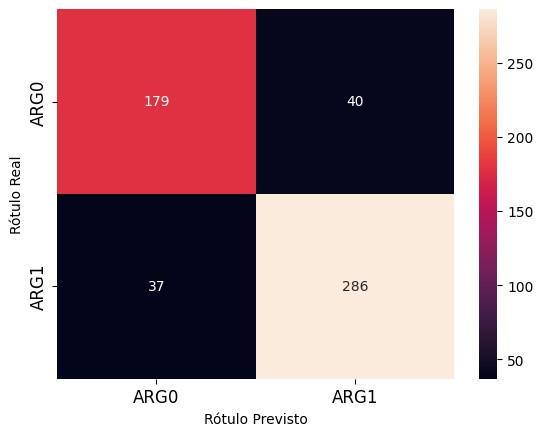
\includegraphics[width=\textwidth]{figure04.jpg}
  \caption{Matriz de confusão do primeiro experimento}
  \label{fig-04}
  \source{Elaborado pelos autores.}
\end{minipage}%
\hfill
\begin{minipage}{.45\textwidth}
  \centering
  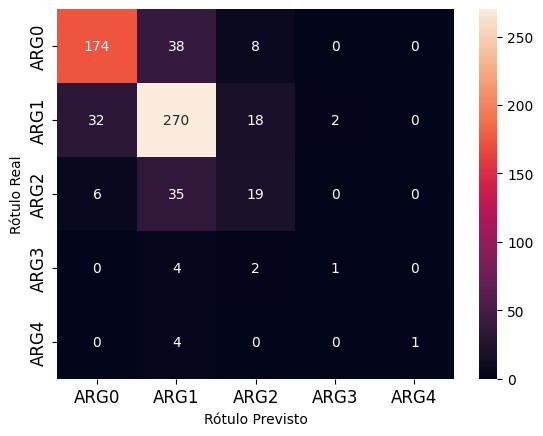
\includegraphics[width=\textwidth]{figure05.jpg}
  \caption{Matriz de confusão do segundo experimento}
  \label{fig-05}
  \source{Elaborado pelos autores.}
\end{minipage}
\end{figure}

As matrizes de confusão para os dois experimentos complementam as
métricas de avaliação apresentadas. No primeiro experimento, o modelo
mostra um bom equilíbrio entre P e R, com 179 (de 219) exemplos de Arg0
e 286 (de 323) exemplos de Arg1 corretamente classificados.

No segundo experimento, o modelo apresentou desequilíbrio em seu
desempenho. As classes Arg0 e Arg1 mantêm uma alta taxa de acerto, ao
passo que Arg2, Arg3 e Arg4 sofrem de baixa precisão e alta taxa de
erros. Essa confusão se deve ao fato de haver um desbalanceamento entre
os tipos de argumentos, conduzindo à classificação conforme a classe
majoritária, a saber, Arg1, conforme já discutido anteriormente.

Ainda, foi feita uma análise sobre o desempenho do modelo considerando
as classes e os \emph{corpora} utilizados nos dois experimentos.

\begin{table}[htpb]
  \centering
  \begin{threeparttable}
    \caption{Resultados do Experimento 1 em função dos \emph{corpora} utilizados.}
    \label{tab-04}
    \begin{tabular}{*{6}{l}}
      \toprule
      Corpora & Classe & P & R & MF & \multicolumn{1}{>{\raggedright\arraybackslash}p{2cm}}{Qnt. de instâncias} \\
      \midrule
      \arrayrulecolor[gray]{.7}
      \multirow{2}{*}{\emph{little prince}} 
        & Arg0 & 0,89 & 0,87 & 0,88 & 119 \\
        & Arg1 & 0,90 & 0,91 & \textbf{0,91} & 151 \\
      \midrule
      \multirow{2}{*}{\emph{news}} 
        & Arg0 & 0,74 & 0,75 & 0,74 & 60 \\
        & Arg1 & 0,87 & 0,86 & \textbf{0,87} & 116 \\
      \midrule
      \multirow{2}{*}{\emph{opisums}} 
        & Arg0 & 0,77 & 0,71 & 0,74 & 34 \\
        & Arg1 & 0,78 & 0,84 & \textbf{0,81} & 43 \\
      \midrule
      \multirow{2}{*}{\emph{sci}} 
        & Arg0 & 0,86 & 1,00 & 0,92 & 6 \\
        & Arg1 & 1,00 & 0,92 & \textbf{0,96} & 13 \\
      \arrayrulecolor{black}
      \bottomrule
    \end{tabular}
    \source{Elaborado pelos autores.}
  \end{threeparttable}
\end{table}

Na \Cref{tab-04}, relativa ao Experimento 1, observa-se que, considerando a
medida de avaliação MF, o modelo apresenta um melhor desempenho para
classificar Arg1 do que Arg0 para todos os \emph{corpora} utilizados.
Tal resultado pode ser explicado pela quantidade de instâncias
analisadas em Arg1 ser maior que Arg0. Ainda sobre a distribuição das
instâncias entre os \emph{corpora}, destaca-se que, apesar do
\emph{corpus sci} apresentar menos instâncias (no total, 19), o
\emph{corpus opisums} apresentou o menor desempenho com relação a MF, a
despeito da quantidade de instâncias (no total, 77). No entanto, é
possível notar que há um bom equilíbrio entre P e R para todos os
\emph{corpora}, indicando resultados consistentes para a classificação
do modelo.

\begin{table}[htpb]
  \centering
  \begin{threeparttable}
    \caption{Resultados do Experimento 2 em função dos \emph{corpora} utilizados.}
    \label{tab-05}
    \begin{tabular}{*{6}{l}}
      \toprule
      Corpora & Classe & P & R & MF & \multicolumn{1}{>{\raggedright\arraybackslash}p{2cm}}{Qnt. de instâncias} \\
      \midrule
      \arrayrulecolor[gray]{.7}
      \multirow{5}{*}{\emph{little prince}} 
        & Arg0 & 0,85 & 0,89 & \textbf{0,87} & 120 \\
        & Arg1 & 0,81 & 0,82 & 0,81 & 151 \\
        & Arg2 & 0,22 & 0,19 & 0,21 & 21 \\
        & Arg3 & 0,50 & 0,20 & 0,29 & 5 \\
        & Arg4 & 1,00 & 0,25 & 0,40 & 4 \\
      \midrule
      \multirow{5}{*}{\emph{news}} 
        & Arg0 & 0,77 & 0,68 & 0,73 & 60 \\
        & Arg1 & 0,74 & 0,86 & \textbf{0,80} & 115 \\
        & Arg2 & 0,57 & 0,39 & 0,46 & 31 \\
        & Arg3 & 0,00 & 0,00 & 0,00 & 1 \\
        & Arg4 & 0,00 & 0,00 & 0,00 & 1 \\
      \midrule
      \multirow{5}{*}{\emph{opisums}} 
        & Arg0 & 0,77 & 0,59 & 0,67 & 34 \\
        & Arg1 & 0,69 & 0,84 & \textbf{0,76} & 43 \\
        & Arg2 & 0,29 & 0,29 & 0,29 & 7 \\
        & Arg3 & 0,00 & 0,00 & 0,00 & 1 \\
        & Arg4 & 0,00 & 0,00 & 0,00 & 0 \\
      \midrule
      \multirow{5}{*}{\emph{sci}} 
        & Arg0 & 0,86 & 1,00 & \textbf{0,92} & 6 \\
        & Arg1 & 1,00 & 0,85 & \textbf{0,92} & 13 \\
        & Arg2 & 1,00 & 1,00 & \textbf{1,00} & 1 \\
        & Arg3 & 0,00 & 0,00 & 0,00 & 0 \\
        & Arg4 & 0,00 & 0,00 & 0,00 & 0 \\
      \arrayrulecolor{black}
      \bottomrule
    \end{tabular}
    \source{Elaborado pelos autores.}
  \end{threeparttable}
\end{table}


Na \cref{tab-05} relativa ao Experimento 2, observa-se que o Arg0 obteve um
melhor desempenho de classificação nos \emph{corpora} \emph{little
prince} e \emph{sci}, com MF de 0,87 e 0,92, respectivamente. Já Arg1
foi melhor classificado nos \emph{corpora news} e \emph{opisums}, com MF
de 0,88 e 0,76, respectivamente. Destaca-se também que no \emph{corpus
news}, Arg3 e Arg4 não foram classificados, apesar de ter um único
exemplo para cada uma dessas classes; o mesmo ocorre para Arg3 no
\emph{corpus opisums}. Em contrapartida,apenas uma única instância de
Arg2 no \emph{corpus sci} foi classificada corretamente pelo modelo.

Ainda com relação à \Cref{tab-05}, é possível inferir que as sentenças dos
\emph{corpora} podem apresentar estruturas argumentais distintas a
depender do domínio e/ou gênero textual a que se vinculam.

Além disso, foi feito um estudo sobre as \emph{features} mais relevantes
para a classificação dos papéis semânticos utilizando o método
\emph{feature importance}. Para tanto, somou-se a importância das
\emph{features} do Experimento 1 (\Cref{fig-06}) e do Experimento 2 (\Cref{fig-07}).

\begin{figure}[h]
  \centering
  \begin{minipage}{.75\textwidth}
  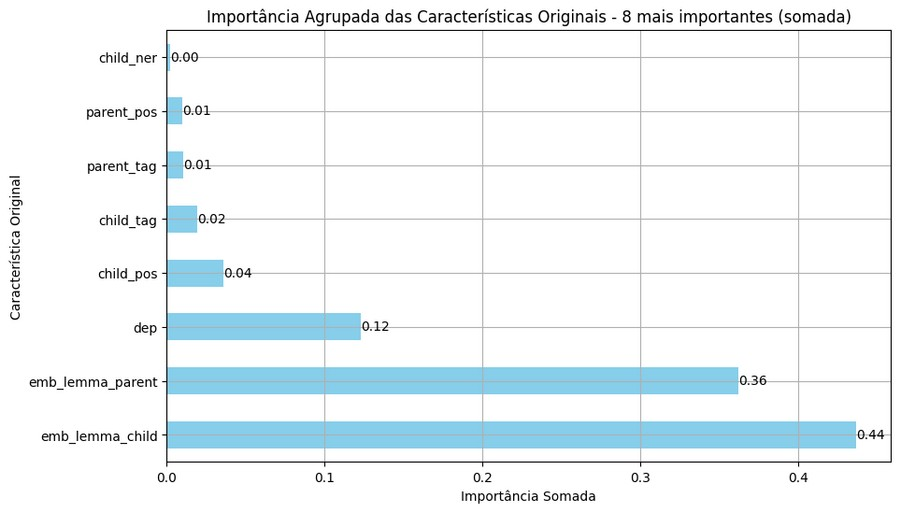
\includegraphics[width=\textwidth]{figure06.jpg}
  \caption{\emph{Features} mais relevantes para o Experimento 1.}
  \label{fig-06}
  \source{Elaborado pelos autores.}
  \end{minipage}
\end{figure}

\begin{figure}[h]
  \centering
  \begin{minipage}{.75\textwidth}
  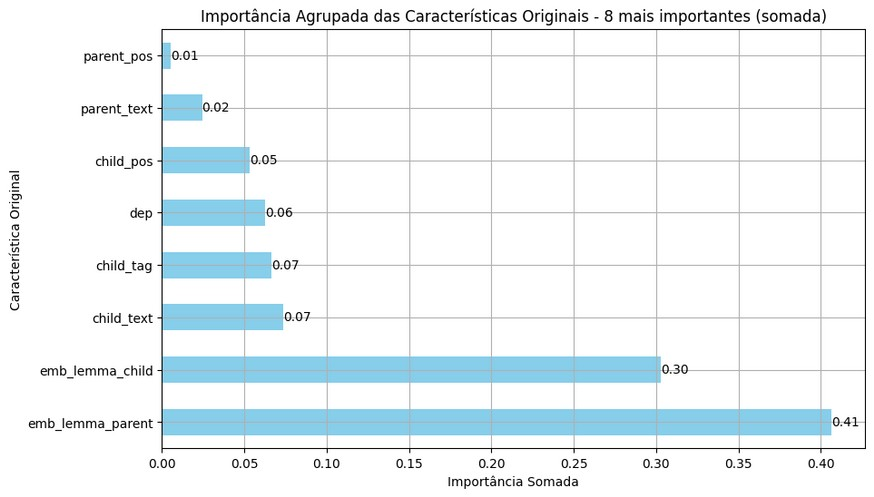
\includegraphics[width=\textwidth]{figure07.jpg}
  \caption{\emph{Features} mais relevantes para o Experimento 2.}
  \label{fig-07}
  \source{Elaborado pelos autores.}
  \end{minipage}
\end{figure}


Na \Cref{fig-06}, observa-se que os \emph{embeddings} dos lemas, tanto de
\emph{parent} quanto de \emph{child}, são particularmente significativos
para o modelo de classificação. No entanto, destaca-se que
\emph{embeddings} são as \emph{features} mais numerosas após a seleção.
Portanto, embora tenham uma grande soma de importância, individualmente,
sua relevância não é tão alta. Já na \Cref{fig-07}, além dos
\emph{embeddings} dos lemas, \emph{child\_tag}, \emph{child\_pos} e
\emph{dep} também se destacam. Nesse sentido, é possível inferir que, no
modelo criado, características de ordens morfossintáticas e sintáticas
são relevantes para a indicação dos papéis semânticos. Ressalta-se que
este tipo de observação é relevante em análises futuras, indicando quais
\emph{features} são mais relevantes em tarefas como a que foi
desenvolvida neste trabalho, além de contrapor o modelo teórico AMR que,
em tese, exclui esses níveis de conhecimento linguístico na
representação do significado e de sua estrutura argumental.

Por fim, foi empregado o método de \emph{shap values} para uma análise
mais profunda. Nesse método, conseguimos analisar como cada
\emph{feature} performa em função dos papéis semânticos observados. É
importante destacar que tal método se difere do
\emph{feature\_importance} por considerar a interação entre as
\emph{features} e a sua influência nas predições específicas. Vale
ressaltar que utilizamos apenas os \emph{shap values} para o conjunto de
treino, tendo em vista que o objetivo da análise é entender quais
padrões o modelo entendeu no seu treinamento como sendo mais
importantes. Para tanto, somaram-se os \emph{shap values} absolutos para
cada uma das \emph{features} originais e tirou-se a média de todas as
instâncias agrupadas pelo argumento para o Experimento 1 (\Cref{fig-08}) e o Experimento 2 (\Cref{fig-09}).

\begin{figure}[h]
  \centering
  \begin{minipage}{.75\textwidth}
  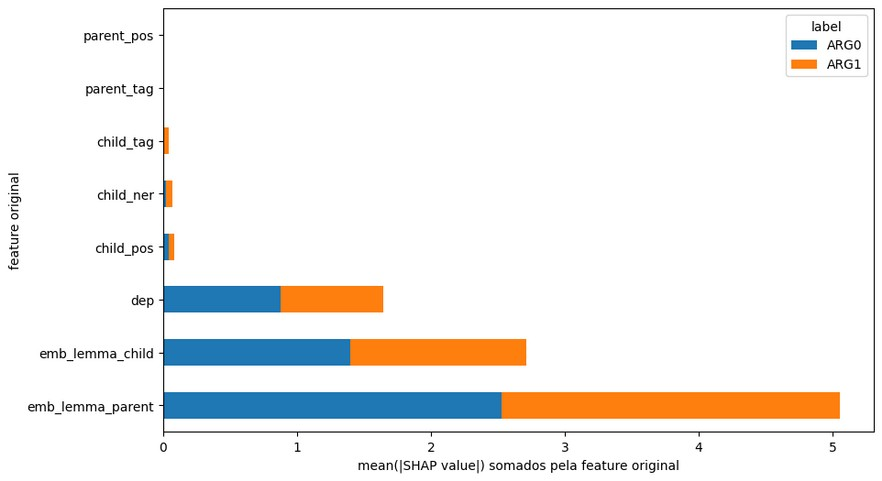
\includegraphics[width=\textwidth]{figure08.jpg}
  \caption{\emph{Features} mais relevantes para o Experimento 1 em função dos argumentos utilizando \emph{shap values}.}
  \label{fig-08}
  \source{Elaborado pelos autores.}
  \end{minipage}
\end{figure}

\begin{figure}[h]
  \centering
  \begin{minipage}{.75\textwidth}
  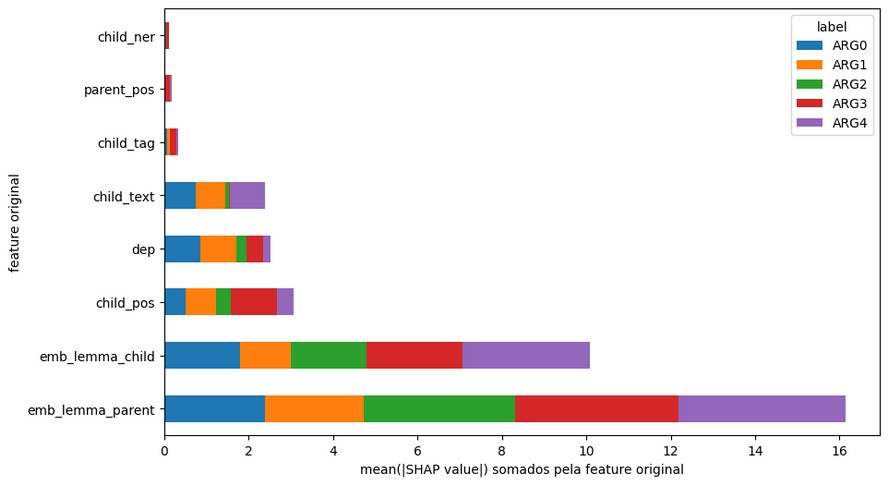
\includegraphics[width=\textwidth]{figure09.jpg}
  \caption{\emph{Features} mais relevantes para o Experimento 2 em função dos argumentos utilizando \emph{shap values}.}
  \label{fig-09}
  \source{Elaborado pelos autores.}
  \end{minipage}
\end{figure}


Na \Cref{fig-08}, evidencia-se que \emph{emb\_lemma\_parent} tem
discretamente maior relevância na classificação automática para Arg1 do
que Arg2, o que é inversamente proporcional para \emph{dep} e
\emph{emb\_lemma\_child}. Quanto a \emph{child\_tag}, \emph{child\_ner}
e \emph{child\_pos}, a relevância é bem baixa nesse cenário para as duas
classes analisadas; ao passo que \emph{parent\_pos} e \emph{parent\_tag}
não apresentaram qualquer relevância para nenhum dos dois papéis
semânticos. Quando o cenário de classificação é ampliado para os Args 0
a 4, o classificador recorre a algumas \emph{features} diferentes
daquelas utilizadas no primeiro experimento. Na \Cref{fig-09}, em especial,
tem-se que \emph{emb\_lemma\_parent} e \emph{emb\_lemma\_child} foram as
\emph{features} com maior relevância na classificação dos papéis
semânticos, sobretudo entre as classes Arg2, Arg3 e Arg4; ao passo que
\emph{child\_text}, que no experimento anterior não havia sido
utilizada, apresenta maior impacto para Arg0, Arg1 e Arg4.
